\documentclass[11pt,a4paper]{article}
\usepackage[utf8]{inputenc}
\usepackage[vietnamese]{babel}
\usepackage{amsmath,amssymb}
\usepackage[version=4]{mhchem}
\usepackage{geometry}
\geometry{top=1.5cm,bottom=1.2cm,left=1.4cm,right=1.4cm,headheight=28pt,headsep=12pt,footskip=18pt}
\usepackage{graphicx}
\usepackage{xcolor}
\usepackage{tabularx}
\usepackage{array}
\usepackage{colortbl}
\usepackage{tikz}
\usepackage{chemfig}
\usepackage{fancyhdr}
\usepackage{enumitem}
\usepackage{multido}
\usepackage{tcolorbox}

\definecolor{hfRed}{HTML}{D32F2F}
\definecolor{hfGreen}{HTML}{8BC390}
\definecolor{mainGreen}{HTML}{2E7D32}
\definecolor{solBlue}{HTML}{1565C0}
\definecolor{tableGreen}{HTML}{E8F5E9}

\usepackage{ex_test}

\pagestyle{fancy}
\fancyhf{}
\renewcommand{\headrulewidth}{0.75pt}
\renewcommand{\headrule}{\hbox to\headwidth{\color{hfGreen}\leaders\hrule height \headrulewidth\hfill}}
\renewcommand{\footrulewidth}{0.75pt}
\renewcommand{\footrule}{\hbox to\headwidth{\color{hfGreen}\leaders\hrule height \footrulewidth\hfill}}

\fancyhead[L]{\small\itshape\color{hfRed}Tài liệu lưu hành nội bộ}
\fancyhead[R]{\small\color{hfRed}Thầy \textbf{TRẦN VĂN THẠNH} - 0777.470.803}

\fancyfoot[L]{\footnotesize\itshape\color{hfRed}CS1: 6/15 Nguyễn Hoàng, P. Kim Long, TP Huế \quad|\quad CS2: 24 Đặng Thái Thân, TP Huế}
\fancyfoot[R]{\small\textbf{\color{hfRed}Trang \thepage}}

\setlength{\parindent}{0pt}
\setlength{\parskip}{2pt}

\begin{document}

\begin{minipage}[t]{0.48\textwidth}
\textbf{SỞ GD\&ĐT THÀNH PHỐ HUẾ}\\
\textbf{TRƯỜNG THPT PHONG ĐIỀN}\\
\textit{ĐỀ CHÍNH THỨC}\\
\textit{(Đề thi có 04 trang)}
\end{minipage}
\hfill
\begin{minipage}[t]{0.48\textwidth}
\raggedleft
\textbf{\color{hfRed}ĐỀ KIỂM TRA CUỐI KÌ I}\\
\textbf{NĂM HỌC 2025 -- 2026}\\
\textbf{MÔN: HÓA HỌC LỚP 11}\\
\textit{Thời gian làm bài: 45 phút (không kể thời gian phát đề)}\\
\textbf{MÃ ĐỀ: 1020}
\end{minipage}

\vspace{4pt}
\noindent
\textit{Họ và tên:} \dotfill \textit{Số báo danh:} \dotfill

\vspace{3pt}
\noindent
\textit{\footnotesize Cho biết nguyên tử khối của các nguyên tố: $\ce{Na} = 23; \ce{Cu} = 64; \ce{Ag} = 108; \ce{Fe} = 56; \ce{S} = 32; \ce{N} = 14; \ce{O} = 16; \ce{H} = 1; \ce{Cl} = 35{,}5; \ce{Br} = 80$.}

\vspace{3pt}
\hrule color{hfGreen} height 0.5pt

\vspace{4pt}
\textit{\small Bảng tín hiệu phổ hồng ngoại của một số nhóm chức cơ bản:}
\begin{center}
\small
\renewcommand{\arraystretch}{1.15}
\begin{tabular}{|l|c|c||l|c|c|}
\hline
\rowcolor{tableGreen}
\textbf{Hợp chất} & \textbf{Liên kết} & \textbf{Số sóng ($\text{cm}^{-1}$)} & \textbf{Hợp chất} & \textbf{Liên kết} & \textbf{Số sóng ($\text{cm}^{-1}$)} \\ \hline
Alcohol & $\ce{O-H}$ & $3500 - 3200$ & Carboxylic & $\ce{C=O}$ & $1760 - 1690$ \\ \cline{1-3}
Ketone & $\ce{C=O}$ & $1715 - 1666$ & acid & $\ce{O-H}$ & $3300 - 2500$ \\ \hline
Aldehyde & $\ce{C-H}$ & $2830 - 2695$ & Ester & $\ce{C=O}$ & $1750 - 1715$ \\ \cline{2-3} \cline{5-6}
& $\ce{C=O}$ & $1740 - 1685$ & & $\ce{C-O}$ & $1300 - 1000$ \\ \hline
\end{tabular}
\end{center}

\vspace{4pt}
{\large\bfseries\color{mainGreen} PHẦN I. Câu trắc nghiệm nhiều phương án lựa chọn (3,0 điểm)}

\textit{Thí sinh trả lời từ câu 1 đến câu 12. Mỗi câu hỏi thí sinh chỉ chọn một phương án.}
\vspace{4pt}
\begin{ex}
Để pha loãng $\ce{H2SO4}$ đặc cách làm nào sau đây đúng?
\begin{center}
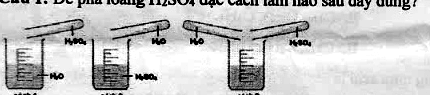
\includegraphics[width=0.55\textwidth]{images_phongdien_ma1020/pha_loang_h2so4_clean.png}
\end{center}
\choice
{cách 1.}
{cách 2.}
{cách 3.}
{cách 1 và 2.}
\loigiai{}
\end{ex}
\begin{ex}
Hợp chất hữu cơ nào sau đây có mạch carbon phân nhánh?
\choice
{$\ce{CH3-CH(OH)-CH3}$}
{$\ce{cyclo-C4H8}$}
{$\ce{CH3-CH(CH3)-CH3}$}
{$\ce{CH3-CH2-CH2-CH2-CH3}$}
\loigiai{}
\end{ex}
\begin{ex}
Kết tinh là phương pháp tách biệt và tinh chế hỗn hợp các chất ....(1) dựa vào độ tan khác nhau và sự thay đổi độ tan của chúng theo .....(2). (1) và (2) lần lượt là
\choice
{rắn -- thời gian.}
{lỏng -- nhiệt độ.}
{rắn -- nhiệt độ.}
{lỏng -- thời gian.}
\loigiai{}
\end{ex}
\begin{ex}
Trước kia, “phẩm đỏ” dùng để nhuộm áo choàng cho các Hồng y giáo chủ được tách chiết từ một loài ốc biển. Đó là một hợp chất có thành phần nguyên tố như sau: 45,70 \%C; 1,90 \%H; 7,60 \%O; 6,70 \%N; 38,10 \%Br. Công thức đơn giản của phẩm đỏ là
\choice
{\ce{C8H4ONBr}.}
{\ce{C4H2ONBr}.}
{\ce{C4H8O2NBr2}.}
{\ce{C2H4ONBr}.}
\loigiai{}
\end{ex}
\begin{ex}
Điền vào khoảng trống bằng cụm từ thích hợp: “Cân bằng hóa học là cân bằng ...(1)... vì tại cân bằng phản ứng ...(2)...”
\choice
{(1) tĩnh; (2) dừng lại.}
{(1) tính; (2) tiếp tục xảy ra.}
{(1) động; (2) tiếp tục xảy ra.}
{(1) động; (2) dừng lại.}
\loigiai{}
\end{ex}
\begin{ex}
Liên kết hóa học trong phân tử $\ce{HNO3}$ là liên kết
\choice
{cộng hóa trị có cực.}
{hydrogen.}
{ion.}
{cộng hóa trị không cực.}
\loigiai{}
\end{ex}
\begin{ex}
Phát biểu nào sau đây đúng khi nói về sự điện li?
\choice
{Sự điện li là quá trình phân li một chất trong nước thành ion.}
{Sự điện li là quá trình phân li một chất dưới tác dụng của dòng điện.}
{Sự điện li quá trình hoà tan một chất vào nước tạo thành dung dịch.}
{Sự điện li thực chất là quá trình oxi hoá - khử.}
\loigiai{}
\end{ex}
\begin{ex}
Cho hình vẽ mô tả thí nghiệm như sau:
\begin{center}
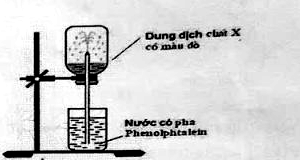
\includegraphics[width=0.38\textwidth]{images_phongdien_ma1020/dai_phun_nuoc_nh3_clean.png}
\end{center}
Hình vẽ mô tả thí nghiệm để chứng minh
\choice
{tính base của $\ce{NH3}$.}
{tính tan nhiều trong nước và tính base của $\ce{NH3}$.}
{tính tan nhiều trong nước của $\ce{NH3}$.}
{tính khử của $\ce{NH3}$.}
\loigiai{}
\end{ex}
\begin{ex}
Dãy nào sau đây gồm các chất đều thuộc dãy đồng đẳng của methane?
\choice
{$\ce{C2H2}, \ce{C3H4}, \ce{C4H6}$.}
{$\ce{CH4}, \ce{C2H2}, \ce{C3H4}$.}
{$\ce{C2H6}, \ce{C3H8}, \ce{C5H12}$.}
{$\ce{CH4}, \ce{C2H6}, \ce{C4H14}$.}
\loigiai{}
\end{ex}
\begin{ex}
Tác nhân chính gây ra hiện tượng mưa acid là
\choice
{$\ce{NH3}, \ce{NO2}$.}
{$\ce{NO_x}, \ce{SO2}$.}
{$\ce{CO}, \ce{SO2}$.}
{$\ce{CO}, \ce{NH3}$.}
\loigiai{}
\end{ex}
\begin{ex}
Ngoài đơn chất nitrogen thì nguyên tố nitrogen còn tồn tại dưới dạng nào?
\choice
{Khoáng vật sodium nitrate ($\ce{NaNO3}$) gọi là diêm tiêu sodium}
{Có trong protein}
{Có trong nucleic acid}
{Có trong diêm tiêu sodium, protein, nucleic acid...}
\loigiai{}
\end{ex}
\begin{ex}
Hợp chất hữu cơ là
\choice
{Hợp chất khó tan trong nước.}
{Hợp chất của cacbon trừ $\ce{CO}, \ce{CO2}, \ce{H2CO3}$, muối cacbonat kim loại...}
{Hợp chất của cacbon và một số nguyên tố khác trừ N, Cl, O.}
{Hợp chất có nhiệt độ sôi cao.}
\loigiai{}
\end{ex}

\vspace{6pt}
{\large\bfseries\color{mainGreen} PHẦN II. Câu trắc nghiệm đúng sai (2,0 điểm)}

\textit{Trong mỗi ý a), b), c), d) ở mỗi câu, thí sinh chọn đúng hoặc sai. Điểm tối đa của 01 câu hỏi là 1 điểm: 01 ý được 0,1đ; 02 ý được 0,25đ; 03 ý được 0,5đ; 04 ý được 1đ.}
\vspace{4pt}
\begin{ex}
Cho khoảng 1 mL hexane vào bát sứ nhỏ, cẩn thận đưa que đóm đang cháy vào bề mặt chất lỏng, hexane bốc cháy cho ngọn lửa màu vàng.
\choiceTF
{ Đốt hexane trong điều kiện thiếu oxygen sinh ra carbon monooxide.}
{ Không nên đốt hexane trong cốc thuỷ tinh do phản ứng này toả ra lượng nhiệt lớn có thể làm vỡ cốc thuỷ tinh.}
{ Phản ứng trên là phản ứng thu nhiệt.}
{ Hexane thành phần chủ yếu của khí dầu mỏ hóa lỏng (LPG).}
\loigiai{}
\end{ex}
\begin{ex}
Thực hiện thí nghiệm tách cồn (ethanol) ra khỏi hỗn hợp cồn -- nước, được mô phỏng như hình sau:
\begin{center}
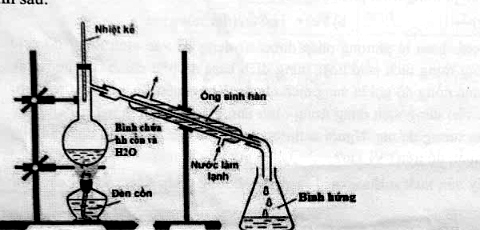
\includegraphics[width=0.6\textwidth]{images_phongdien_ma1020/thi_nghiem_chung_cat_clean.png}
\end{center}
\choiceTF
{ Đầu nước vào và nước ra của ống sinh hàn có thể được đặt ngược lại.}
{ Thí nghiệm đã sử dụng phương pháp chưng cất.}
{ Phương pháp tách ethanol và nước dựa trên sự khác nhau về khối lượng riêng.}
{ Độ cồn của sản phẩm sẽ lớn hơn so với độ cồn ban đầu do sản phẩm thu được tinh khiết hơn lẫn ít nước hơn cồn ban đầu.}
\loigiai{}
\end{ex}

\vspace{6pt}
{\large\bfseries\color{mainGreen} PHẦN III: Câu trắc nghiệm yêu cầu trả lời ngắn (2,0 điểm)}

\textit{Thí sinh làm tròn kết quả đến hàng phần mười.}
\vspace{4pt}
\begin{ex}
Một cơ sở nhỏ sản xuất tinh dầu sả từ thân và lá sả tươi. Sau khi đun sôi hỗn hợp sả với nước, người ta thu được một hỗn hợp gồm nước và tinh dầu sả, trong đó tinh dầu sả không tan trong nước, nhẹ hơn nước và còn lẫn một lượng nhỏ tạp chất rắn từ nguyên liệu thực vật. Để tách riêng và tinh chế tinh dầu sả đạt độ tinh khiết cao, cách lựa chọn và ưu tiên thứ tự sử dụng các phương pháp hóa học nào sau đây là hợp lí nhất?
\begin{enumerate}[label=\arabic*.,leftmargin=20pt,itemsep=0pt]
\item Làm khô và tinh chế bằng kết tinh nhằm loại bỏ tạp chất còn sót lại.
\item Chưng cất thường để thu hỗn hợp
\item chiết để tách tinh dầu khỏi nước
\end{enumerate}
\par\textit{Trả lời:} \dotfill
\loigiai{}
\end{ex}
\begin{ex}
Cho lần lượt các chất sau $\ce{FeS}, \ce{Fe3O4}, \ce{Fe2O3}, \ce{FeO}, \ce{Fe(OH)2}, \ce{Fe(OH)3}, \ce{FeSO4}, \ce{Fe2(SO4)3}$ tác dụng với dung dịch $\ce{H2SO4}$ đặc nóng. Số phản ứng oxi hóa -- khử là?
\par\textit{Trả lời:} \dotfill
\loigiai{}
\end{ex}
\begin{ex}
Người ta xác định được \% khối lượng các nguyên tố trong vitamin C: $\%C = 40{,}91\%$; $\%H = 4{,}545\%$; $\%O = 54{,}545\%$. Số nguyên tử của C, H, O trong CTPT vitamin C. biết $M_{\text{vitamin C}} = 176$.
\par\textit{Trả lời:} \dotfill
\loigiai{}
\end{ex}
\begin{ex}
Hợp chất 3-methylpentane có công thức cấu tạo dưới đây:
\[
\ce{CH3 - CH2 - CH(CH3) - CH2 - CH3}
\]
Khi cho 3-methylpentane tác dụng với khí chlorine thu được số đồng phân cấu tạo là dẫn xuất monochloro tối đa là
\par\textit{Trả lời:} \dotfill
\loigiai{}
\end{ex}

\vspace{6pt}
{\large\bfseries\color{mainGreen} PHẦN IV: Tự luận (3,0 điểm)}

\textit{Thí sinh trình bày lời giải chi tiết vào phần giấy làm bài thi.}
\vspace{4pt}
\textbf{Câu 1: (0,5 điểm)} Trình bày các luận điểm chính của Thuyết cấu tạo hóa học?

\vspace{2pt}
\multido{}{6}{\noindent\dotfill\par\vspace{2pt}}

\vspace{4pt}
\textbf{Câu 2: (0,5 điểm)} Trình bày các bước gọi tên thay thế của Alkane phân nhánh?

\vspace{2pt}
\multido{}{6}{\noindent\dotfill\par\vspace{2pt}}

\vspace{4pt}
\textbf{Câu 3: (0,5 điểm)} Hoàn thành các phương trình phản ứng sau:
\begin{enumerate}[label=\alph*),leftmargin=25pt,itemsep=2pt]
\item $\ce{Cu(OH)2 + H2SO4(đặc, nóng) ->}$
\item $\ce{Fe + H2SO4(đặc, nóng) ->}$
\end{enumerate}

\vspace{2pt}
\multido{}{5}{\noindent\dotfill\par\vspace{2pt}}

\vspace{4pt}
\textbf{Câu 4: (0,5 điểm)} Chuẩn độ acid- base là phương pháp được sử dụng để xác định nồng độ acid hoặc base chưa biết nồng độ bằng dung dịch acid hoặc dung dịch base đã biết chính xác nồng độ. Khi đó dung dịch đã biết chính xác nồng độ gọi là dung dịch chuẩn. Khi chuẩn độ, người ta thêm từ từ dung dịch đựng trong burette vào dung dịch đựng trong bình tam giác. Tại điểm mà hai chất tác dụng vừa đủ với nhau gọi là điểm tương đương. Người ta thường dựa vào đặc điểm nào để nhận biết điểm tương đương trong phép chuẩn độ trên? Vì sao?

\vspace{2pt}
\multido{}{7}{\noindent\dotfill\par\vspace{2pt}}

\vspace{4pt}
\textbf{Câu 5: (1,0 điểm)} Một nhà máy sản xuất sulfuric acid áp dụng phương pháp tiếp xúc với các giai đoạn chính sau:
\begin{itemize}[leftmargin=20pt,itemsep=0pt]
\item Đốt Sulfur hoặc quặng pyrite tạo $\ce{SO2}$
\item Oxi hóa $\ce{SO2}$ thành $\ce{SO3}$ trên xúc tác $\ce{V2O5}$
\item Hấp thụ $\ce{SO3}$ để thu sulfuric acid
\end{itemize}
Trong quá trình vận hành, nhà máy phải đồng thời đảm bảo hiệu suất cao, tiết kiệm năng lượng và giảm thiểu ô nhiễm môi trường.

1. Xét phản ứng oxi hóa: $\ce{2SO2(g) + O2(g) <=> 2SO3(g)},\quad (\Delta H < 0)$
\begin{enumerate}[label=\alph*),leftmargin=20pt,itemsep=0pt]
\item Cho biết phản ứng trên là thu nhiệt hay tỏa nhiệt.
\item Giải thích vì sao trong thực tế không tiến hành phản ứng ở nhiệt độ quá cao, mặc dù tốc độ phản ứng sẽ tăng.
\end{enumerate}
2. Để tăng hiệu suất tổng hợp $\ce{SO3}$ người ta phải điều chỉnh các yếu tố: Nhiệt độ, Áp suất, Nồng độ $\ce{SO2}$ và $\ce{O2}$ như thế nào?

\vspace{2pt}
\multido{}{10}{\noindent\dotfill\par\vspace{2pt}}

\vspace{6pt}
\begin{center}
\textbf{\large ---------- HẾT ----------}
\end{center}

\end{document}
